% explanations http://www.math.umbc.edu/~rouben/beamer/
\documentclass{beamer}

\usepackage{style/beamertheme_amsterdam}
% \renewcommand{\labelitemi}{$\vcenter{\hbox{\tiny$\bullet$}}$}

\beamertemplatenavigationsymbolsempty
\usepackage{natbib}
\usepackage{tikz}
\usepackage{pbox}
\usepackage{listings}
\usepackage[export]{adjustbox}
\lstset{language=Java} 
\usepackage{mdframed}
\mdfdefinestyle{IndexFrame}{%
    linecolor=blue,
    outerlinewidth=2pt,
    roundcorner=20pt,
    innertopmargin=\baselineskip,
    innerbottommargin=\baselineskip,
    innerrightmargin=20pt,
    innerleftmargin=20pt
    innermargin=10pt
    }
\graphicspath{ {images/} }

\newenvironment{nscenter}
 {\parskip=0pt\par\nopagebreak\centering}
 {\par\noindent\ignorespacesafterend}

\newcommand\blfootnote[1]{%
  \begingroup
  \renewcommand\thefootnote{}\footnote{#1}%
  \addtocounter{footnote}{-1}%
  \endgroup
}

\renewcommand{\footnoterule}{%
  \kern -3pt
  \hrule width \textwidth height 0.1pt
  \kern 2pt
}

\title{Designing an Index for ZooDB}
%\subtitle{}
\author{Jonas Nick \& Bogdan Vancea}
\begin{document}
  \frame{\titlepage}
  \begin{frame}
    \frametitle{Outline}
    \tableofcontents[hideallsubsections]
  \end{frame}

  \begin{section}{Introduction}
    \begin{frame}
      % \frametitle{ZooDB}
      \vspace{-4em}
      \hspace{-2em}
      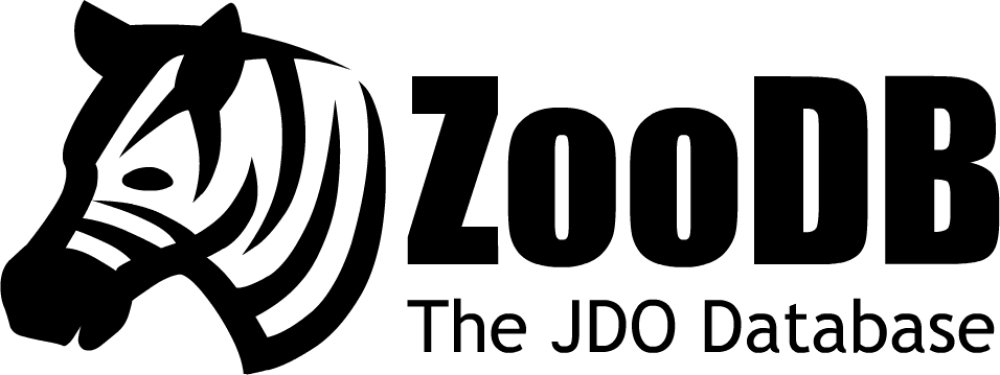
\includegraphics[scale=0.1]{images/zoodb_logo.png}
      \vspace{3em}
      \hspace{2em}
      \begin{itemize}
        \item an open source object database written in Java
        \item JDO standard compliant
        \item 4 times faster than competitor db4o
          % on pole position
        \item \url{zoodb.org}
      \end{itemize}

    \end{frame}
    \begin{frame}
      \frametitle{Database Index}
      \begin{block}{}
        \textbf{Key-Value} data structure \\
        \begin{enumerate}
        \item \textbf{fast} retrieval 
        \item \textbf{ordered} iteration
        \item stored in a \textbf{file}
        \end{enumerate}
      \end{block}
      \vspace{1em}
      % Example: \lstinline|ZooJdoHelper.createIndex(pm, Person.class, "name", false);|
      \pause
      \texttt{ZooJdoHelper.createIndex(pm, Person.class, "name", false);}
      \pause
      \begin{center}
      \fbox{\parbox[t][3em][c]{0.29\textwidth}{Attribute Index\\ Value $\rightarrow$ Object-ID} }
      \pause
      \fbox{\parbox[t][3em][c]{0.29\textwidth}{ObjectID Index\\ OID $\rightarrow$ Diskpos} }
      \fbox{\parbox[t][3em][c]{0.29\textwidth}{Free Space Index \\ Page-ID $\rightarrow$ TxID} }
      \end{center}
    \end{frame}

    \begin{frame}
      \frametitle{B+ Tree}
      \pause
      \vspace{-1em}
      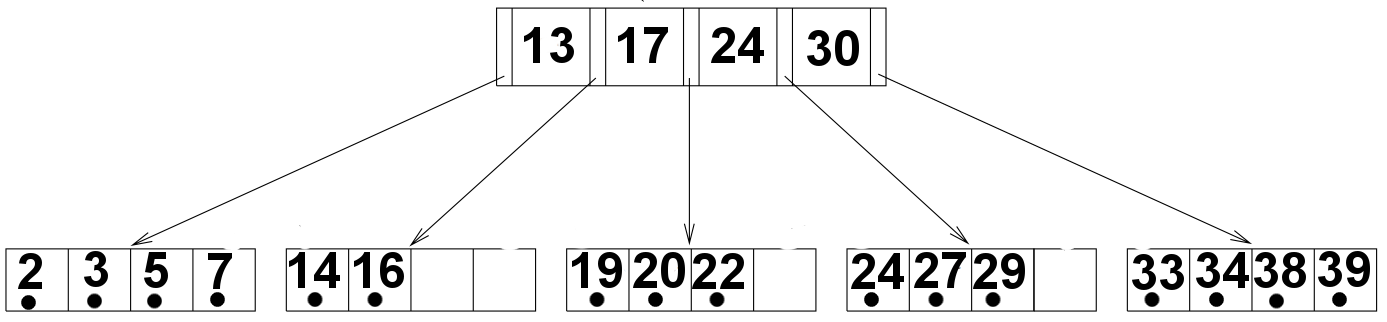
\includegraphics[scale=0.2]{B+Tree.png}
      \blfootnote{\tiny Images adapted from Database Management Systems by Ramakrishnan and Gehrke.}
      \vspace{2em}
      \begin{itemize}
        \item Inner node contains keys and children pointer, \\leaf contains keys and values.
        \pause
        \item \textbf{Node fills one disk page.}
        \pause
        \item Node has maximum and minimum number of entries.
          % over, underfull
          % after operations rebalancing
      \end{itemize}
    \end{frame}

    \begin{frame}
      \frametitle{Example: insert $(8,v)$}
      \blfootnote{\tiny Images adapted from Database Management Systems by Ramakrishnan and Gehrke.}
      \vspace{-1em}
      \begin{center}
      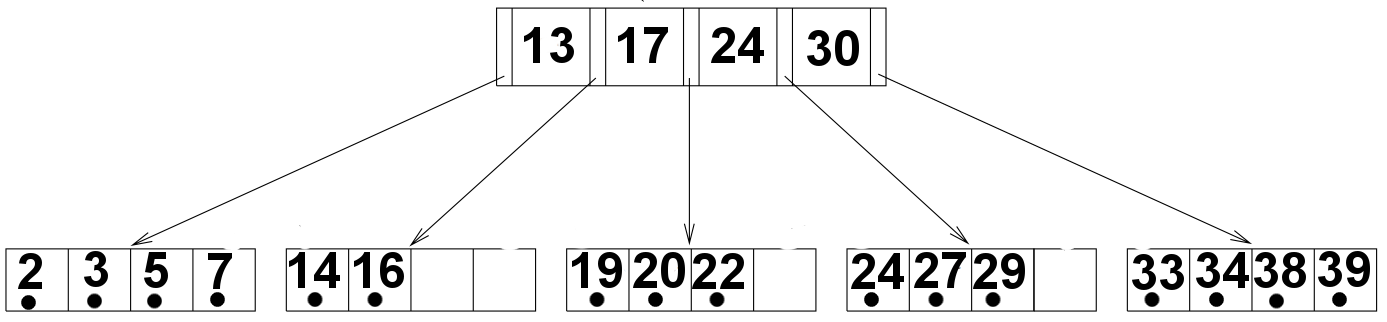
\includegraphics[scale=0.17]{B+Tree.png}
      \end{center}
      \pause
      \vspace{-2em}
      \begin{figure}[!ht]
        \centering
        \begin{center}
          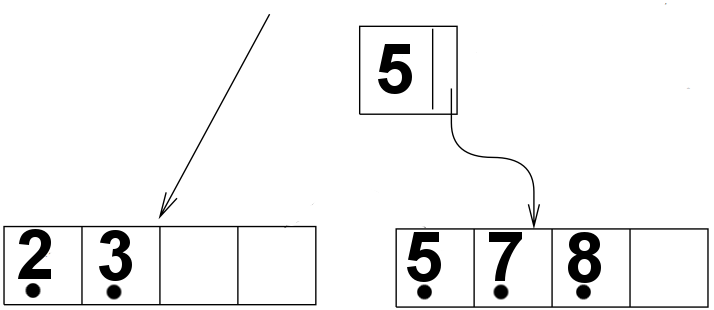
\includegraphics[valign=t,scale=0.15]{B+Tree_op1.png}
          \quad
          \pause
          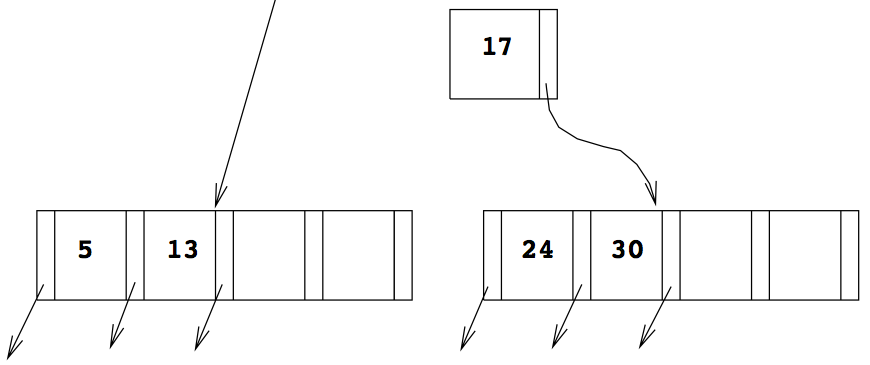
\includegraphics[valign=t,scale=0.15]{B+Tree_op2.png}
        \end{center}
      \end{figure}
      \pause
      \begin{center}
      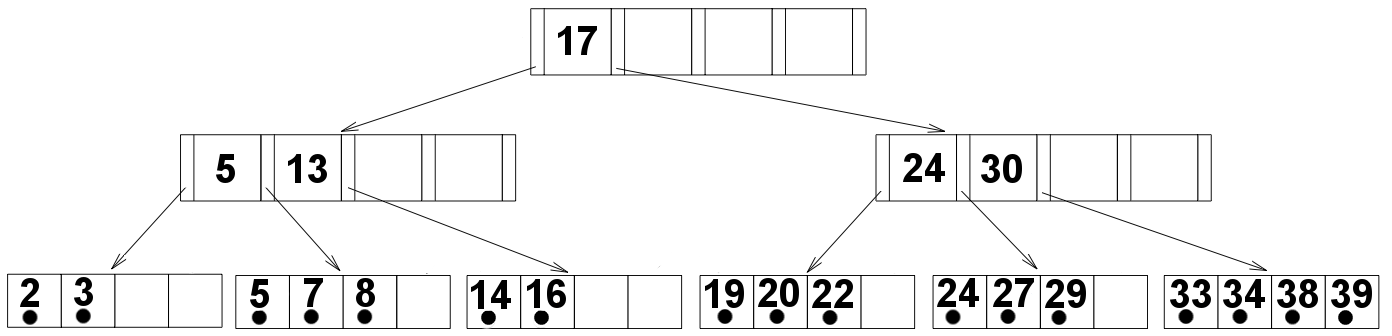
\includegraphics[scale=0.2]{B+Tree_op3.png}
      \end{center}
    \end{frame}
  \end{section}

    \begin{frame}
      \frametitle{B+ Tree}
      % \vspace{-1em}
      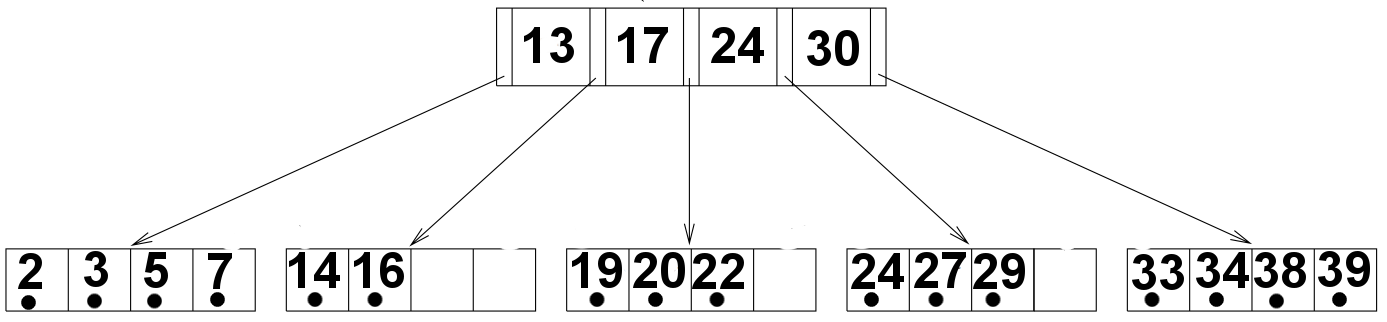
\includegraphics[scale=0.2]{B+Tree.png}
      \blfootnote{\tiny Images adapted from Database Management Systems by Ramakrishnan and Gehrke.}
      \vspace{1em}
      \begin{itemize}
        \item Inner node contains keys and children pointer, \\leaf contain keys and values.
        \item \textbf{Node fills one disk page.}
        \item Node has maximum and minimum number of entries.
          % over, underfull
          % after operations rebalancing
        \pause
        \item Rebalancing
          \begin{itemize}
            \item on insert: split
            \item on delete: redistribute or merge
          \end{itemize}
        \pause
        \item Insert, remove, search are logarithmic.
      \end{itemize}
    \end{frame}


  \begin{section}{Goals \& Challenges}
    % 3908 loc + 2665 loc of test
    \begin{frame}
      \frametitle{Goals}
        \begin{itemize}
          \item faster B+ tree index
          \pause
          \item key unique and key-value unique
          \begin{itemize}
            \item Ex. insert (1,1), (1,2)
          \end{itemize}
          \pause
          \item range query iterators
          \pause
          \item buffer manager to allow caching
          \begin{itemize}
            \item fetches pages 
          \end{itemize}
          \pause
          \item prefix sharing
        \end{itemize}
    \end{frame}

    \begin{frame}
      \frametitle{Prefix Sharing}
      \setbeamercovered{invisible}
      \begin{block} {Exploit common prefix}
      \hspace*{\fill}
      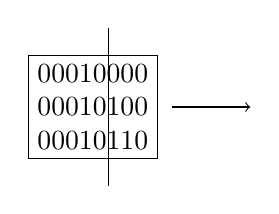
\begin{tikzpicture}
        \node[draw,align=left] at (0,0) {00010000\\ 00010100\\ 00010110};
        \onslide<2->{\draw (0.2,-1) -- (0.2,1);}
        \onslide<2->{\draw [->] (1,0) -- (2,0);}
      \end{tikzpicture}
      \pause
      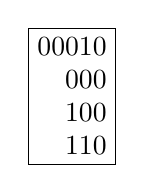
\begin{tikzpicture}
        \onslide<3->{\node[draw,align=right] at (0,0) {00010\\ 000\\100\\110};}
      \end{tikzpicture}
      \hspace*{\fill}
      \end{block}
      \pause
      \pause
        \begin{itemize}
            \item variable number of key-value entries per node 
            \pause
            \item prefix determines
            \begin{itemize}
              \item if can be split without underflow
              \pause
              \item if can be merged without overflow
              \pause
              \item the number redistributions
            \end{itemize}
        \end{itemize}    
    \end{frame}

    \begin{frame}
      \frametitle{Challenges}
        \begin{itemize}
          \item runtime dominated by disk access
          \pause
          \begin{itemize}
            \item prefer fewer nodes
            \pause
            \item rarely modify nodes
          \end{itemize}
          \pause
          \item New features are costly.
          \pause
          \item Textbook algorithms need to be adapted.
          \pause
          \begin{enumerate}
            \item not optimized for practical scenarios
            \pause
            % Pointers, inner node and leaf order different 
            \item do not cover duplicates nor prefix sharing
            % dont know max number of keys
          \end{enumerate}
          \pause
          \item low-level implementation optimizations
        \end{itemize}
    \end{frame}
  \end{section}

  \begin{section}{The new Index Implementation}
    \begin{frame}
        \frametitle{Index Implementation}
        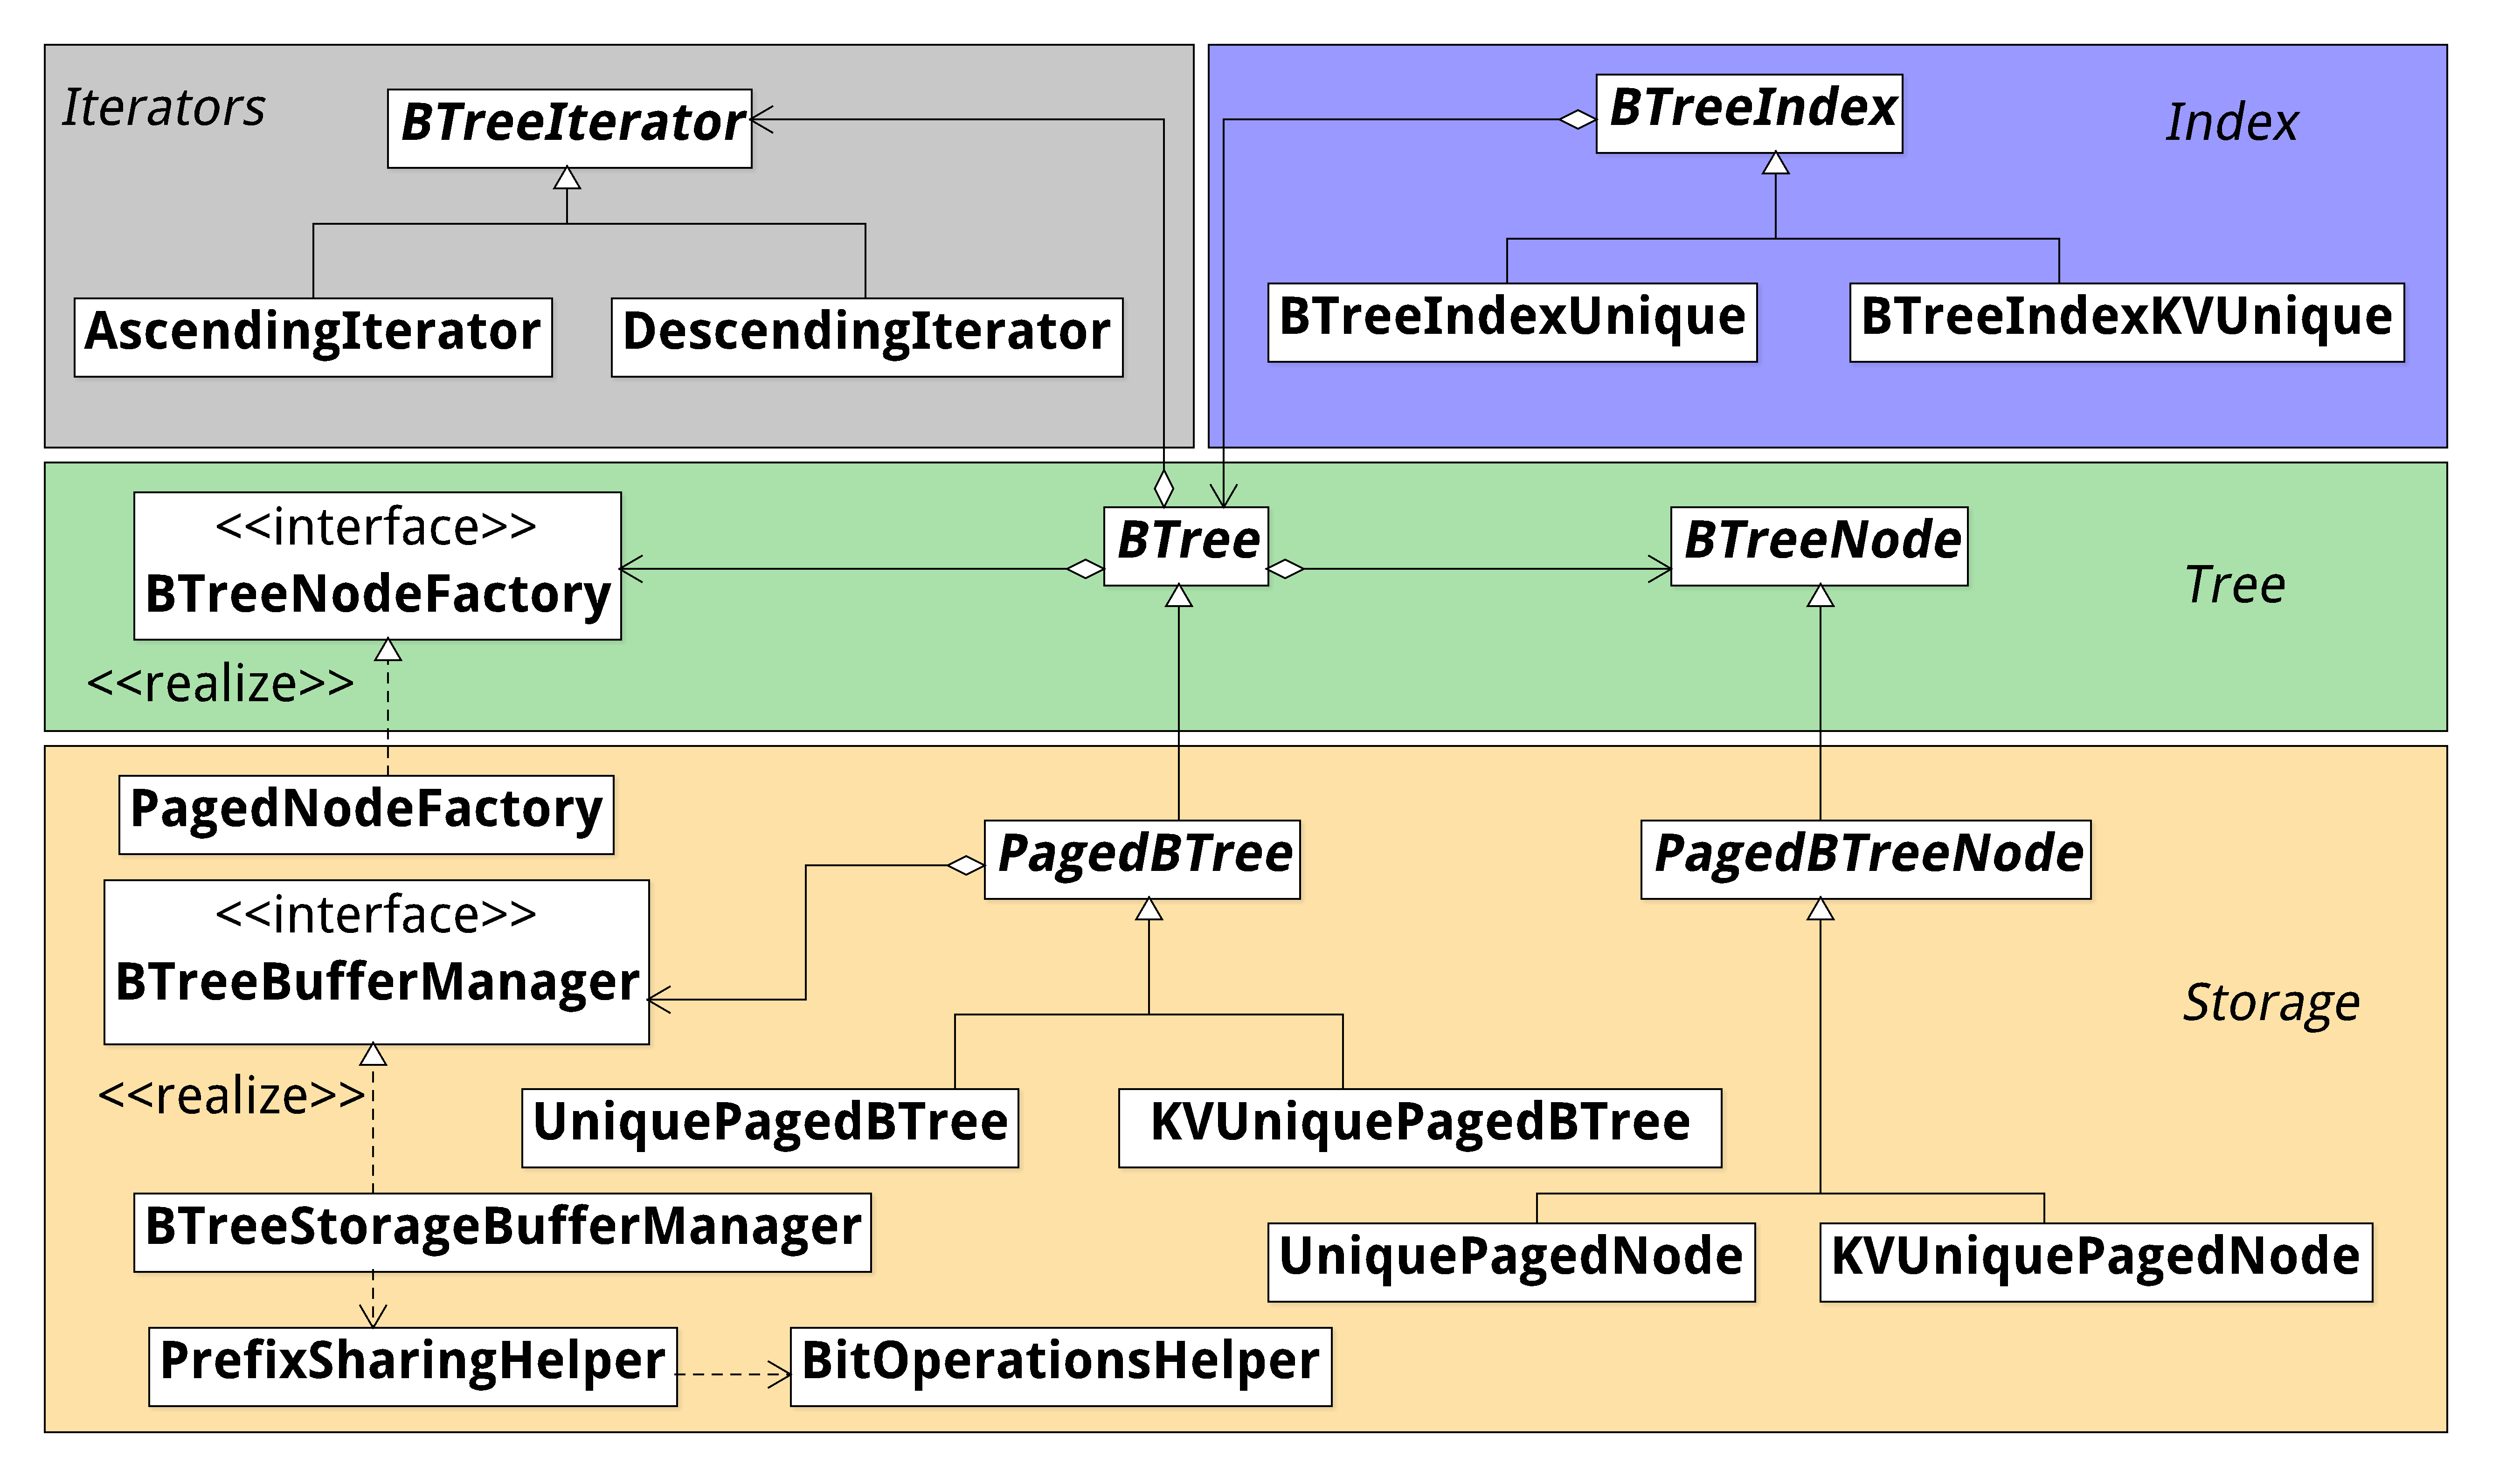
\includegraphics[scale=0.065]{ZooDBClassDiagram} 
        % one general BTree
        % paged, unique and non-unique 
        % only BTreeNode
        % iterators
    \end{frame}

    \begin{frame}
        \frametitle{Operations}
        \begin{itemize}
        \item Search - Similar to normal B+ Tree
        \pause
        \item Insert overflow
            \begin{itemize}
            \item attempt to redistribute values to left sibling before creating a new node
            \end{itemize}
        \pause
        \item Delete underflow
            \begin{itemize}
            \item check if possible to merge with left or right neighbour
            \item check if possible to split current node between left and right
            \item redistribute from left or right
            \end{itemize}
        \pause
        \item Write
            \begin{itemize}
              \item only write dirty nodes
              \item prefix encoding
            \end{itemize}
        \end{itemize}
    \end{frame}
  \end{section}

  \begin{section}{Benchmarks}
    % \begin{frame}
    %   \frametitle{Microbenchmarks}
    %   \begin{figure}
    %     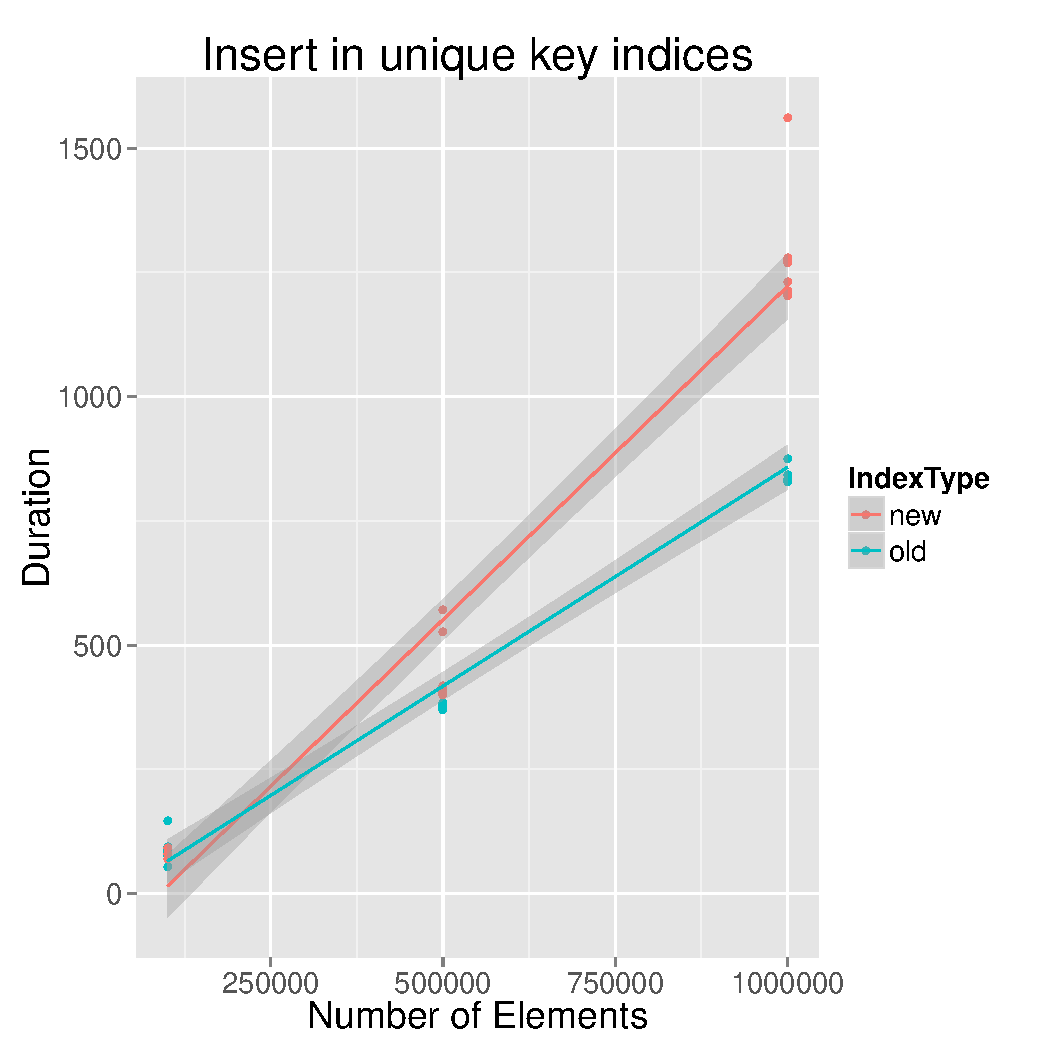
\includegraphics[scale=0.28]{images/unique_random_insert.pdf}
    %     \quad
    %     \pause
    %     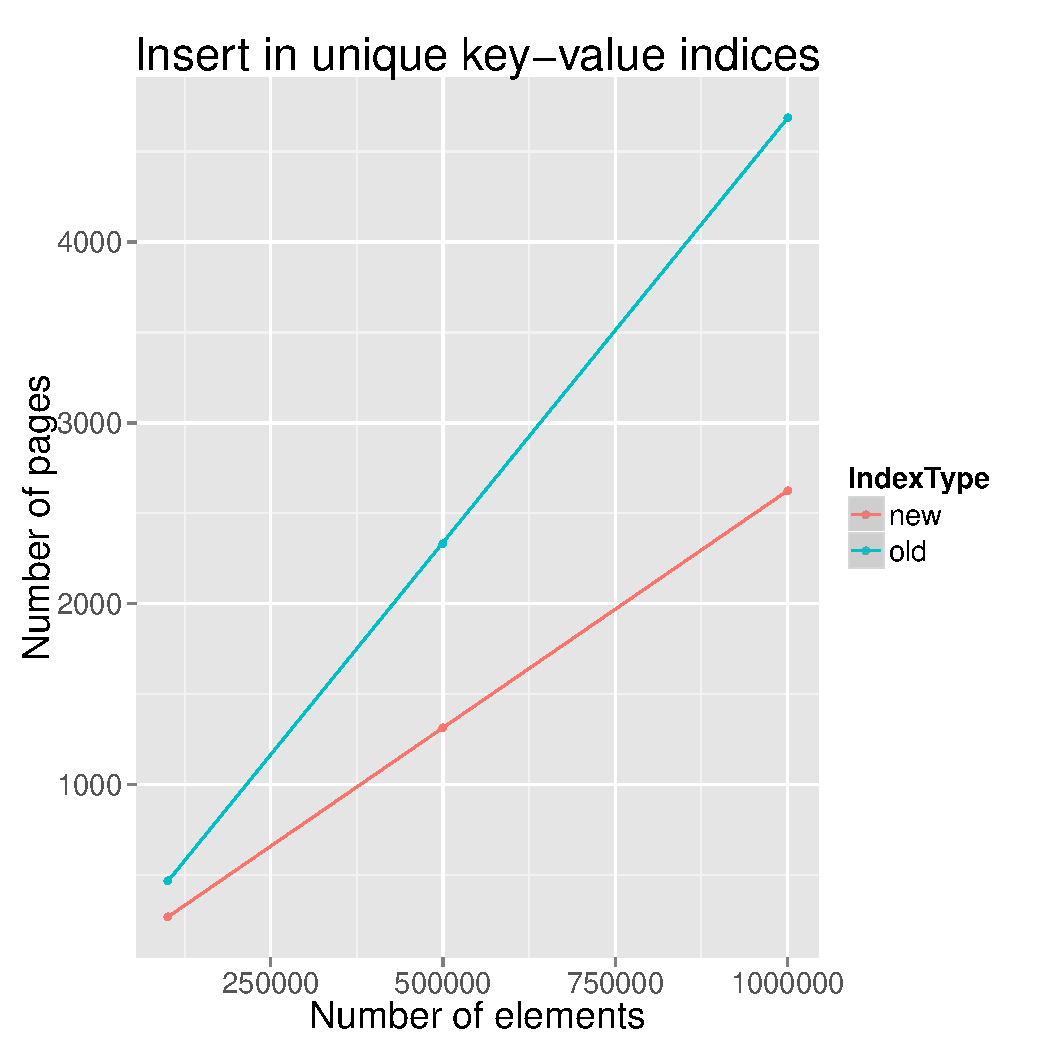
\includegraphics[scale=0.28]{images/nonUnique_random_insert_nodes.pdf}
    %   \end{figure}
    %   \pause
    %     \begin{itemize}
    %       \item in every microbenchmark the new index is significantly slower
    %       \item in most microbenchmarks there s a significantly lower number of nodes
    %       % insert duration (for Unique-random) and nodes (for nonUnique-random), search nonUnique (or increasing) and hope that its fast
    %       % mention that random is worst case
    %       % write?
    %     \end{itemize}
    % \end{frame}

    
    \begin{frame}
      \frametitle{Microbenchmarks}
        
        \begin{block}{Duration}
        
        \end{block}
       \begin{tabular}{| l | l | l | l |}
        \hline
        Operation & Baseline (No prefix sharing) & Prefix sharing \\ \hline 
        Search & 1 & 0.9 - 1.1  \\ \hline 
        Insert & 1 & 1.6 - 2.8  \\ \hline 
        Delete & 1 & 1.45 - 2.9  \\ \hline 
      \end{tabular}
      
        \begin{block}{
        Size of B+ tree}
        \end{block}
       \begin{tabular}{| l | l | l | l |}
        \hline
        Operation & Baseline (No prefix sharing) & Prefix sharing \\ \hline 
        Insert & 1 & 0.5 - 1.1  \\ \hline 
        Delete & 1 & 0.5 - 0.75  \\ \hline 
      \end{tabular}
    \end{frame}
    
    % \begin{frame}
    %   \frametitle{Microbenchmarks}
    %   \begin{figure}
    %     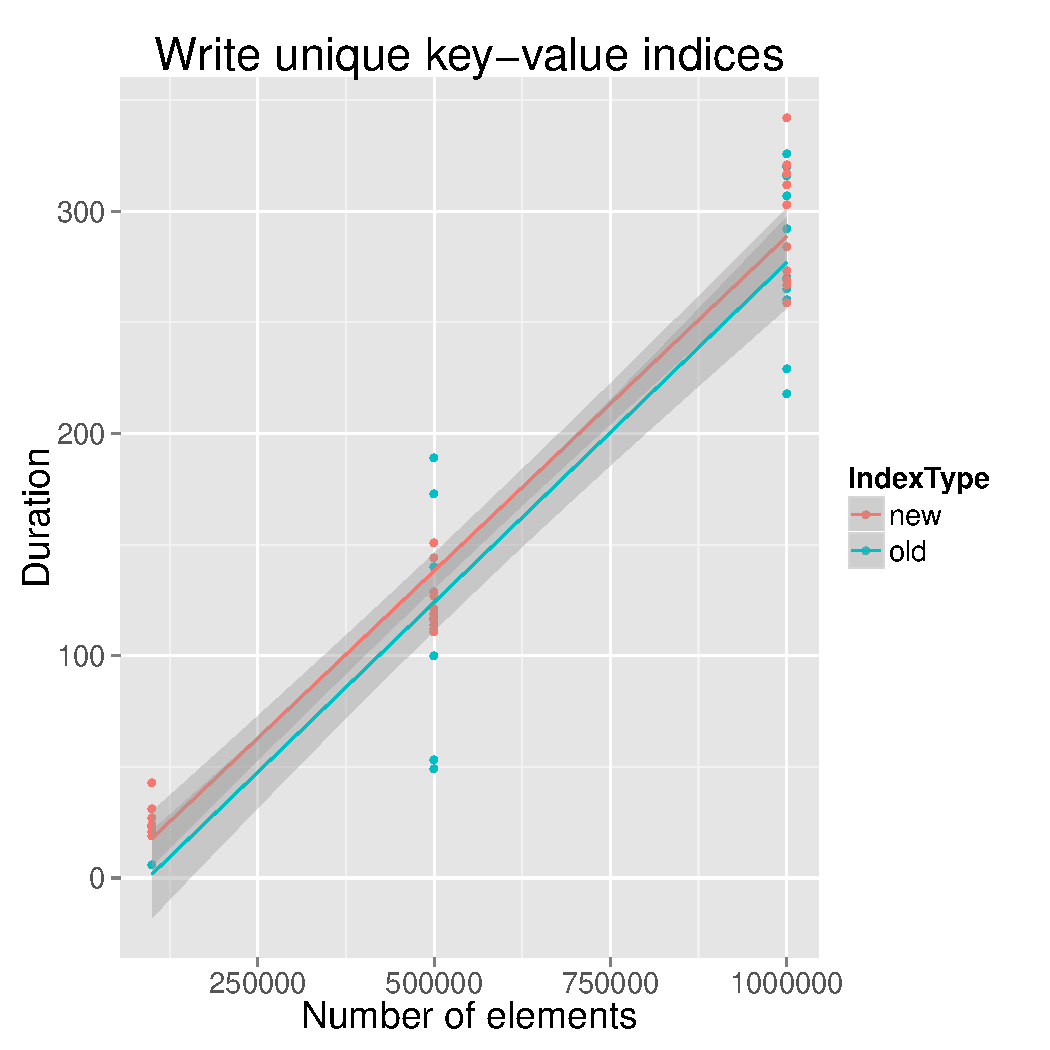
\includegraphics[scale=0.3]{images/nonUnique_random_write.pdf}
    %   \end{figure}
    % \end{frame}

    \begin{frame}
      \frametitle{StackOverflow Data Import}
        \begin{itemize}
        \item Real-world workload consisting of importing StackOverflow data: users, posts, comments and votes     
        \item 3 key unique attribute indexes and 9 key-value unique indexes
        \end{itemize}
    \end{frame}
    
    \begin{frame}
      \frametitle{StackOverflow Import - Index Sizes}
      
        \begin{columns}[c]
        \column{1.5in}
        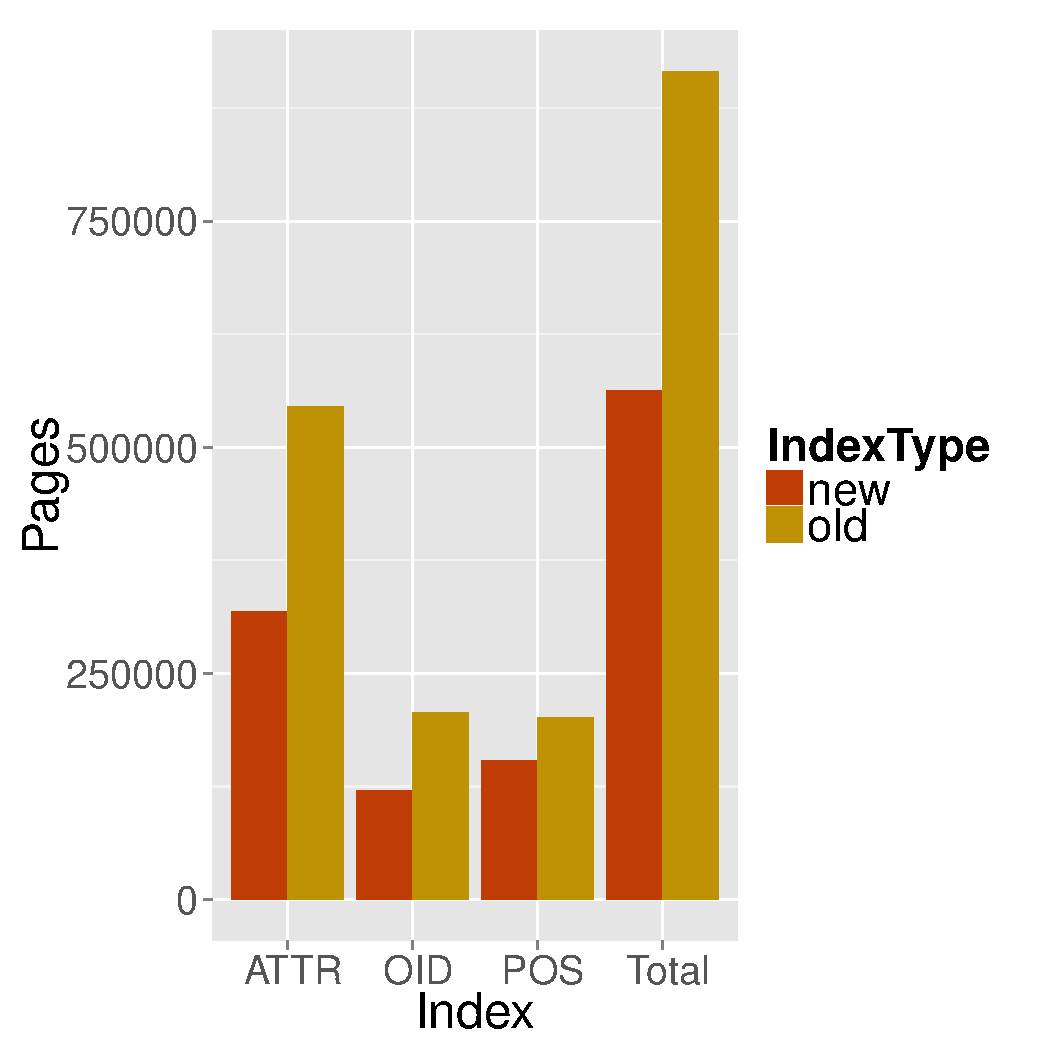
\includegraphics[scale=0.28]{images/SO_sizes.pdf} 
        
        \column{1.5in}
        \begin{tabular}{| l | l |}
            \hline
            Index & Space saving (\%) \\ \hline 
            Atrribute & 41.6   \\ \hline 
            OID & 41.5   \\ \hline 
            POS & 23.1   \\ \hline
            Total & 38.5   \\ \hline 
        \end{tabular}
        
        \end{columns}
        %   \pause
        %   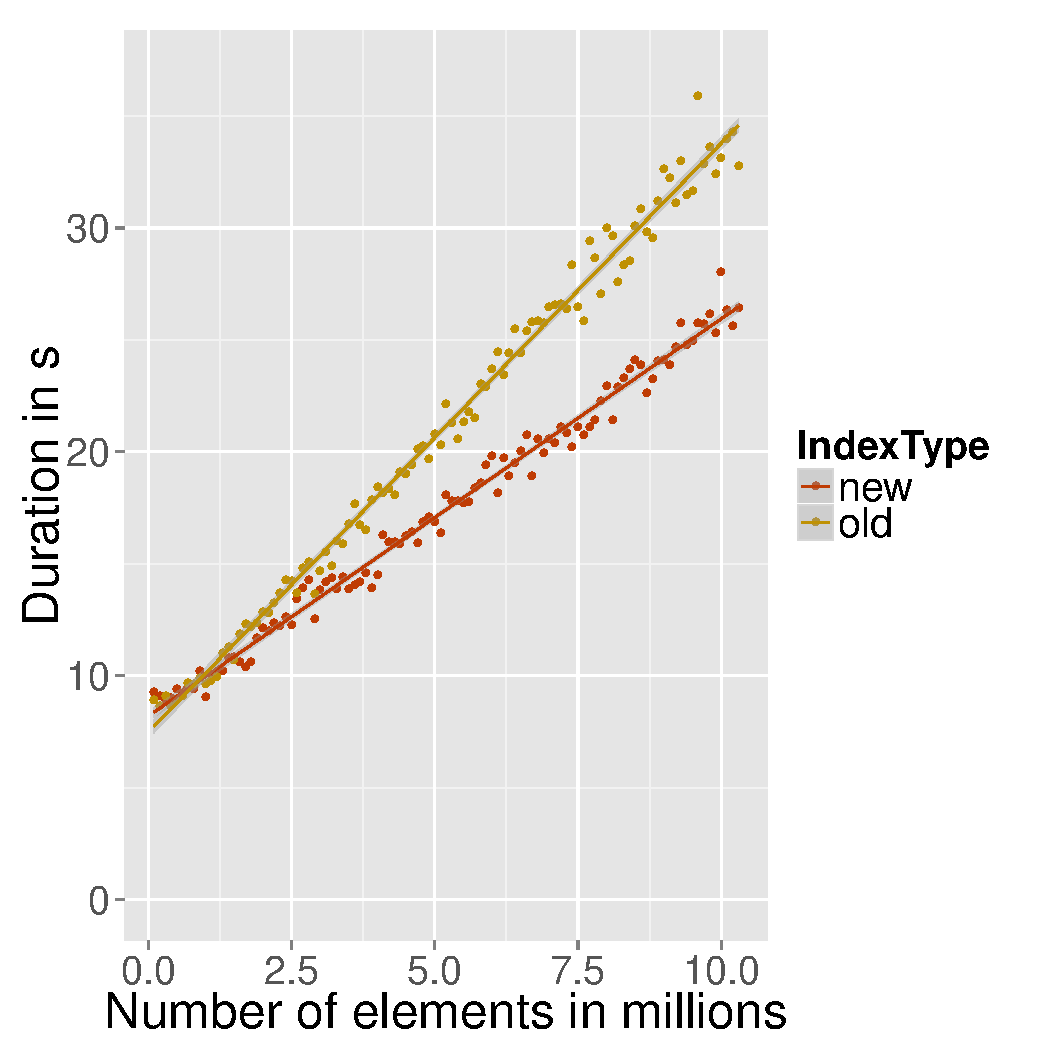
\includegraphics[scale=0.28]{images/SO_commit_duration.pdf}
    \end{frame}
    
    \begin{frame}{StackOverflow Import - Commit times}
        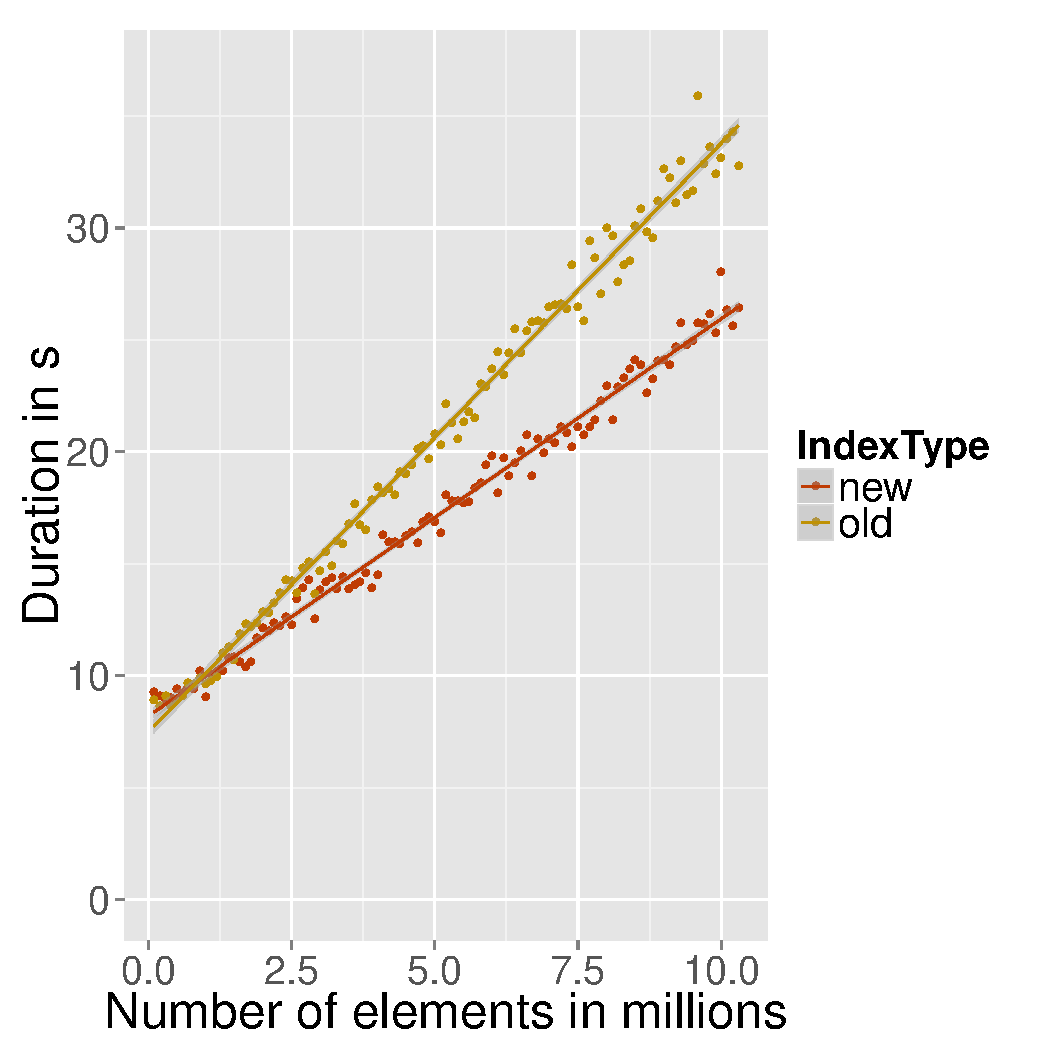
\includegraphics[scale=0.28]{images/SO_commit_duration.pdf}
    \end{frame}
  \end{section}

%   \begin{frame}
%     \frametitle{Summary}
%       \begin{itemize}
%         \item ...
%       \end{itemize}
%   \end{frame}

%   \begin{frame}
%     \frametitle{Outlook}
%       \begin{itemize}
%         \item ...
%       \end{itemize}
%   \end{frame}

  \begin{frame}
    \frametitle{Q\&A}
      \begin{itemize}
        \item Thank you for your attention!
        \item Questions ?
      \end{itemize}
  \end{frame}

\end{document}
